% Options for packages loaded elsewhere
\PassOptionsToPackage{unicode}{hyperref}
\PassOptionsToPackage{hyphens}{url}
%
\documentclass[
]{article}
\usepackage{amsmath,amssymb}
\usepackage{lmodern}
\usepackage{iftex}
\ifPDFTeX
  \usepackage[T1]{fontenc}
  \usepackage[utf8]{inputenc}
  \usepackage{textcomp} % provide euro and other symbols
\else % if luatex or xetex
  \usepackage{unicode-math}
  \defaultfontfeatures{Scale=MatchLowercase}
  \defaultfontfeatures[\rmfamily]{Ligatures=TeX,Scale=1}
\fi
% Use upquote if available, for straight quotes in verbatim environments
\IfFileExists{upquote.sty}{\usepackage{upquote}}{}
\IfFileExists{microtype.sty}{% use microtype if available
  \usepackage[]{microtype}
  \UseMicrotypeSet[protrusion]{basicmath} % disable protrusion for tt fonts
}{}
\makeatletter
\@ifundefined{KOMAClassName}{% if non-KOMA class
  \IfFileExists{parskip.sty}{%
    \usepackage{parskip}
  }{% else
    \setlength{\parindent}{0pt}
    \setlength{\parskip}{6pt plus 2pt minus 1pt}}
}{% if KOMA class
  \KOMAoptions{parskip=half}}
\makeatother
\usepackage{xcolor}
\IfFileExists{xurl.sty}{\usepackage{xurl}}{} % add URL line breaks if available
\IfFileExists{bookmark.sty}{\usepackage{bookmark}}{\usepackage{hyperref}}
\hypersetup{
  hidelinks,
  pdfcreator={LaTeX via pandoc}}
\urlstyle{same} % disable monospaced font for URLs
\usepackage{graphicx}
\makeatletter
\def\maxwidth{\ifdim\Gin@nat@width>\linewidth\linewidth\else\Gin@nat@width\fi}
\def\maxheight{\ifdim\Gin@nat@height>\textheight\textheight\else\Gin@nat@height\fi}
\makeatother
% Scale images if necessary, so that they will not overflow the page
% margins by default, and it is still possible to overwrite the defaults
% using explicit options in \includegraphics[width, height, ...]{}
\setkeys{Gin}{width=\maxwidth,height=\maxheight,keepaspectratio}
% Set default figure placement to htbp
\makeatletter
\def\fps@figure{htbp}
\makeatother
\setlength{\emergencystretch}{3em} % prevent overfull lines
\providecommand{\tightlist}{%
  \setlength{\itemsep}{0pt}\setlength{\parskip}{0pt}}
\setcounter{secnumdepth}{-\maxdimen} % remove section numbering
\usepackage{enumitem}
\usepackage{amsfonts}

\usepackage[
    paperheight=11in,
    paperwidth=8.5in,
    left=1in,
    right=1in,
    top=1in,
    bottom=1in
]{geometry}

\setlist[itemize,1]{label=$\bullet$}
\setlist[itemize,2]{label=$\circ$}
\setlist[itemize,3]{label=$\star$}

% Override tightlist to be less tight
\renewcommand{\tightlist}{%
  \setlength{\itemsep}{1pt}\setlength{\parskip}{1pt}}
\ifLuaTeX
  \usepackage{selnolig}  % disable illegal ligatures
\fi

\author{}
\date{}

\begin{document}

\hypertarget{investigate-whether-predictit-markets-are-well-calibrated}{%
\section{Investigate whether PredictIt markets are well
calibrated}\label{investigate-whether-predictit-markets-are-well-calibrated}}

\hypertarget{academic-research-prior-work}{%
\subsection{Academic Research Prior
Work}\label{academic-research-prior-work}}

Existing work on whether prediction markets are well calibrated.

\href{page_clemen_ej_2013.pdf}{DO PREDICTION MARKETS PRODUCE
WELL-CALIBRATED PROBABILITY FORECASTS?. Page, Clemen 2013}

They use the following approach:

\begin{itemize}
\tightlist
\item
  Local Regression Estimator (sampled at 100 discrete price points, 0.10
  sized window)
\item
  Sample on transactions
\item
  Sample 10 per market.
\item
  597 competitions, 1787 markets, 512612 transactions
\item
  InTrade dataset
\end{itemize}

\hypertarget{replication}{%
\subsection{Replication}\label{replication}}

For adapting to available predictit market data. We can:

\begin{itemize}
\tightlist
\item
  Keep N samples per contract (or market).
\item
  Sample on price changes?

  \begin{itemize}
  \tightlist
  \item
    Or maybe hourly
  \end{itemize}
\item
  Local Regression Estimator

  \begin{itemize}
  \tightlist
  \item
    Or just use simple windowed average for initial implementation
  \end{itemize}
\end{itemize}

\hypertarget{implementation}{%
\subsection{Implementation}\label{implementation}}

\begin{itemize}
\tightlist
\item
  Determine contracts where outcome can be determined from final market
  price.

  \begin{itemize}
  \tightlist
  \item
    Get final market price + check if \textgreater{} 0.98
  \item
    Get final day from db, check last day price
  \end{itemize}
\item
  Aggregate samples per contract.

  \begin{itemize}
  \tightlist
  \item
    python?
  \end{itemize}
\item
  Merge + compute calibration curve
\end{itemize}

\hypertarget{initial-results}{%
\subsection{Initial Results}\label{initial-results}}

We try to sample in a method similar by simpler compare to Page, Clemen
by using an exponential weighting function on each of 100 discrete price
points to compute the emperical resolution frequencies. We look at both
sampling on active contracts on each day, and also take their approach
of collecting a fixed number of samples per market. This normalizes for
markets with different \# of contracts and trading days.

Initial results on nonbinary markets suggests there is a significant
midrange segment where long contracts are overpriced.

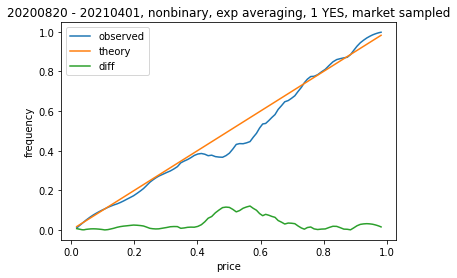
\includegraphics[width=\textwidth,height=1.5625in]{pos_nonbinary_market_sampled.png}
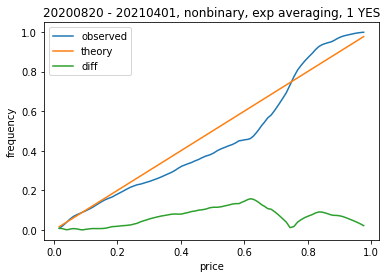
\includegraphics[width=\textwidth,height=1.5625in]{pos_nonbinary.png}

That being said, a significant portion of the data came from Biden
cabinet markets, where many cabinet picks were not confirmed. These
events were highly correlated, and removing them from the picture
weakens the correlation.

We start to see the trend of contracts with price \textgreater0.8 being
underpriced.

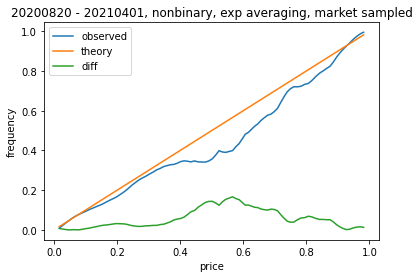
\includegraphics[width=\textwidth,height=1.5625in]{all_nonbinary_market_sampled.png}
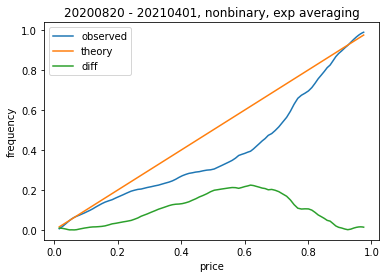
\includegraphics[width=\textwidth,height=1.5625in]{all_nonbinary.png}

Binary markets seem reasonable well calibrated with the exception of
tail probabilities. Probably combination of large ``risk-free'' rate as
well as 2020 election markets being Trump conspiracy biased.

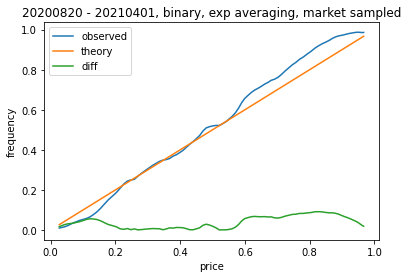
\includegraphics[width=\textwidth,height=1.5625in]{_binary_market_sampled.png}
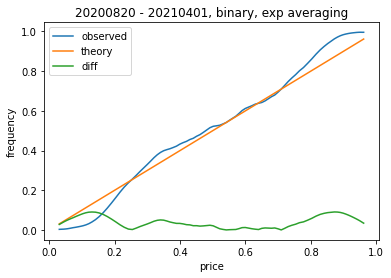
\includegraphics[width=\textwidth,height=1.5625in]{_binary.png}

Finally, it seems like the explanation for the difference between market
sampled and day sampled has more to do with the normalization over
number of days rather than normalizing over \# of contracts. (should say
nonbinary)

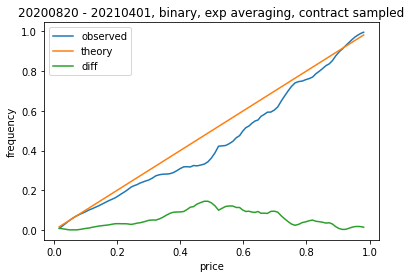
\includegraphics[width=\textwidth,height=1.5625in]{all_nonbinary_contract_sampled.png}
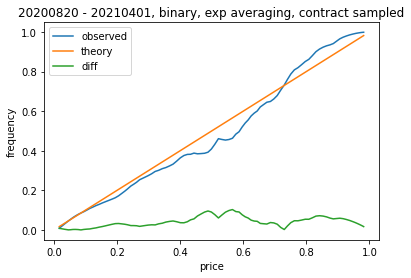
\includegraphics[width=\textwidth,height=1.5625in]{pos_nonbinary_contract_sampled.png}

Confidence intervals (resampling half of markets, assumes markets
reasonable independent)

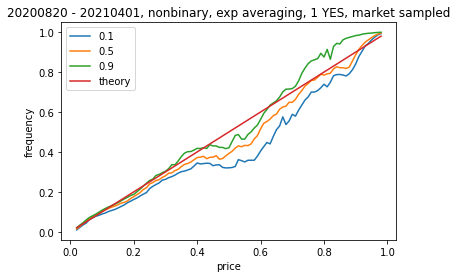
\includegraphics[width=\textwidth,height=1.5625in]{pos_nonbinary_market_sampled_conf.png}

\hypertarget{theory}{%
\subsection{Theory}\label{theory}}

$$1 + 4 = \alpha$$

\end{document}
